
%% include the next line for the long version of the paper
\newcommand{\longpaper}{}



\newcommand{\draftpaper}{}

% detect interpreter: pdflatex or latex

\newif\ifpdf
\ifx\pdfoutput\undefined
  \pdffalse
\else
  \pdftrue
\fi

\newif\iflong
\ifx\longpaper\undefined
  \longfalse
\else
  \longtrue
\fi

\newif\ifdraft
\ifx\draftpaper\undefined
  \draftfalse
\else
  \drafttrue
\fi

\newif\ifverbose
\ifx\verbosepaper\undefined
  \verbosefalse
\else
  \verbosetrue
\fi


% use document class IROS with any paper size:

%%\iflong
%%  \documentclass[a4]{epirob}
  \documentclass[a4]{article}
%%\else
%%  \documentclass[a4paper]{IROS}
%%\fi

%%\documentclass[a4paper]{article}

%%\documentstyle{doublespace}

\usepackage{setspace}


\ifpdf
  \usepackage{graphicx}
\else
  \usepackage[dvips]{graphicx}
\fi

\usepackage{psfig}

\setstretch{2.0}

\begin{document} 

\onecolumn


% create the title header:

\title{Better Vision Through Manipulation}
%%\title{Active Vision is more than just Moving Cameras}
%%\title{Towards Manipulation-Driven Vision}

%%\iflong
%%  \author{Giorgio Metta$^{*,**}$
%%        \and
 %%         Paul Fitzpatrick$^{**}$}
%%  \affiliation{\rm $^{*}$LIRA-Lab, DIST \\
 %%              University of Genova \\
 %%               Viale F. Causa, 13 \\
  %%              16145 Genova, Italy \\
  %%         \and
 %%             $^{**}$MIT AI Lab\\
 %%            200 Technology Square \\
 %%            Cambridge, MA 02139 US }
%%\else
%%\author{Paul M. Fitzpatrick$^{*}$ and Giorgio Metta$^{*,\dagger}$}
%%\affiliation{
%%$^{*}$MIT AI Lab -- Massachussetts Institute of Technology -- USA\\
%%$^{\dagger}$Lira Lab, DIST -- University of Genova -- Italy
%%}
%%\fi

%%\maketitle\thispagestyle{empty} % don't forget \thispagestyle{empty}, otherwise you'll get page numbering

\ifdraft
  \pagenumbering{arabic}
  \thispagestyle{plain}
  \pagestyle{plain}
\fi

% write the abstract with the Abstract-environment:

\iflong
\begin{abstract}
\else
\begin{Abstract}
\fi
 
For the purposes of manipulation, we would like to know what parts of
the environment are physically coherent ensembles -- that is, which
parts will move together, and which are more or less independent.  It
takes a great deal of experience before this judgement can be made
from purely visual information.  This paper develops active strategies
for acquiring that experience through experimental manipulation, using
tight correlations between arm motion and optic flow to detect both
the arm itself and the boundaries of objects with which it comes into
contact.  We argue that following causal chains of events out from
the robot's body into the environment allows for a very natural
developmental progression of visual competence, and relate this idea 
to results in neuroscience.

\ifverbose
For the purpose of understanding development we would like to present
causality as a possible principle to frame a number of neural science
results coherently. We will show how this can lead also to an
implementation in an artificial system following the epigenetic
approach. To this purpose we will show different levels of causal
linkages, or instances of the general principle, which allow tasks of
increasing complexity to be implemented.  Action and the physical
interaction of the robot with the environment play a fundamental role.
In an ecological perspective, the role of this physical interaction
for developing categorization and object undestanding is emphasized.
\fi

%%{\bf \em
%%\iflong
%%(long version)
%%\else
%%(short version)
%%\fi
%%}

\iflong
\end{abstract}
\else
\end{Abstract}
\fi


% ...and start writing!
\chapter{Introduction}

\section{Definition of terms}

The YARP library supports transmission of a stream of
user data across
various protocols -- TCP, UDP, MCAST (multi-cast), shared memory, QNX
message passing -- insulating a user of the library from the
idiosyncratic details of the network technology used.  We call these
these low-level protocols the ``Carriers'', to distinguish them from
the higher-level protocols we will be concerned with here.

For the purposes of YARP, communication takes place throogh
``Connections'' between named entities called ``Ports''.
These form a directed graph, the ``YARP Network'', where Ports are the nodes,
and Connections are the edges.

Each Port is assigned a unique name, such as ``/motor/wheels/left''.  
Every Port is registered by name with
a ``name server''.  The goal is to ensure that if you know the name
of a Port, that is all you need in order to be able to 
communicate with it from any machine.

The purpose of Ports is to move ``Content'' (sequences of bytes representing 
user data) from
one thread to another (or several others) across process and machine
boundaries.  The flow of data can be manipulated and monitored
externally (e.g. from the command-line) at run-time.  In other words,
the edges in the YARP Network are entirely mutable.

Ports are specialized into InputPorts and OutputPorts.
Any OutputPort can send Content to any number of InputPorts.  Any
InputPort can receive Content from any number of OutputPorts.  If an
OutputPort is configured to send Content to an InputPort, they are
said to have a Connection.  Connections can be freely added or 
removed, and may use different Carriers.

The YARP name server is a server that tracks information about ports.
It indexes this information by name, playing a role analogous to
DNS on the internet.
%
To communicate with a port, the properties of that port need to be
known (the machine it is running on, the socket it is listening on,
the carriers it supports).  The YARP name server offers a convenient
place to store these properties, so that only the name of the port is
needed to recover them.
%
The protocol for communicating with the name server
and its operation is specified in section \ref{sect:name-protocol}.

Here are the specifications available in this document:
%
\begin{itemize}

\item Properties of a YARP network.

\item Properties of the YARP utility.

\item Properties of the YARP name server and the protocol used 
for communicating with it.

\item Properties of ports and the protocol used
for communicating with them.

\end{itemize}


\section{Properties of a YARP network}

A YARP network consists of the following entities: a set of
ports, a set of connections, a set of names, a name server, and a set
of registrations.

\begin{itemize} \pflist

\item Every port has a unique name.

\item Every connection has a source port and a target port.

\item Each port maintains a list of all connections for which it
is the target port.

\item Each port maintains a list of all connections for which it
is the source port.

\item There is a single name server in a YARP network.

\item The name server maintains a list of registrations.  Each 
registration contains information about a single port, identified
by name.

\end{itemize}


\noindent
Communication within a YARP network can occur between two ports,
between a port and the name server, between a port and an
external entity, and between the name server and an external entity.


\begin{itemize} \pflist

\item Communication between two ports occurs if and only if there
is a connection between them.  That communication uses the
``connection protocol''.

\item Connections involving a port can be created, destroyed, or
queried by communication between an external entity and that port.
This is done by sending ``port commands'' using the YARP
connection protocol.

\item Ports communicate with the name server using the 
``YARP name server protocol''.  Such communication is needed
to create, remove, and query registrations.

\item External entities can also use the YARP name server protocol
to query the name server.

\end{itemize}

\noindent
The standard YARP companion utility can be used to create a
name server, and also to act as an external entity for querying and
modifying the YARP network.



\section{The experimental platform}

This work is implemented on the robot Cog, an upper torso humanoid
\cite{brooks99cog}.  The robot has previously been applied to tasks
such as visually-guided pointing \cite{Marjanovic-96-SAB}, and
rhythmic operations such as turning a crank or driving a slinky
\cite{williamson98neural}.  Cog has two arms, each of which has six
degrees of freedom -- two per shoulder, elbow, and wrist.  The joints
are driven by series elastic actuators \cite{williamson95series} --
essentially a motor connected to its load via a spring (think strong
and torsional rather than loosely coiled).  The arm is not designed to
enact trajectories with high fidelity.  For that a very stiff arm is
preferable.  Rather, it is designed to perform well when interacting
with a poorly characterized environment, where collisions are frequent
and informative events.

\begin{figure}[tbh]
\centerline{
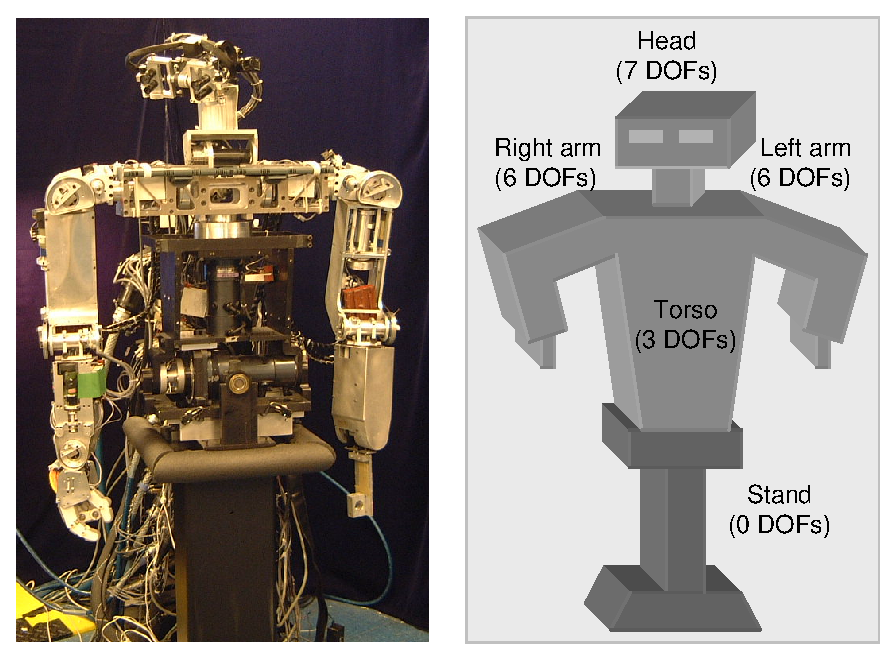
\includegraphics[width=\columnwidth]{cog-schematic.eps}
%%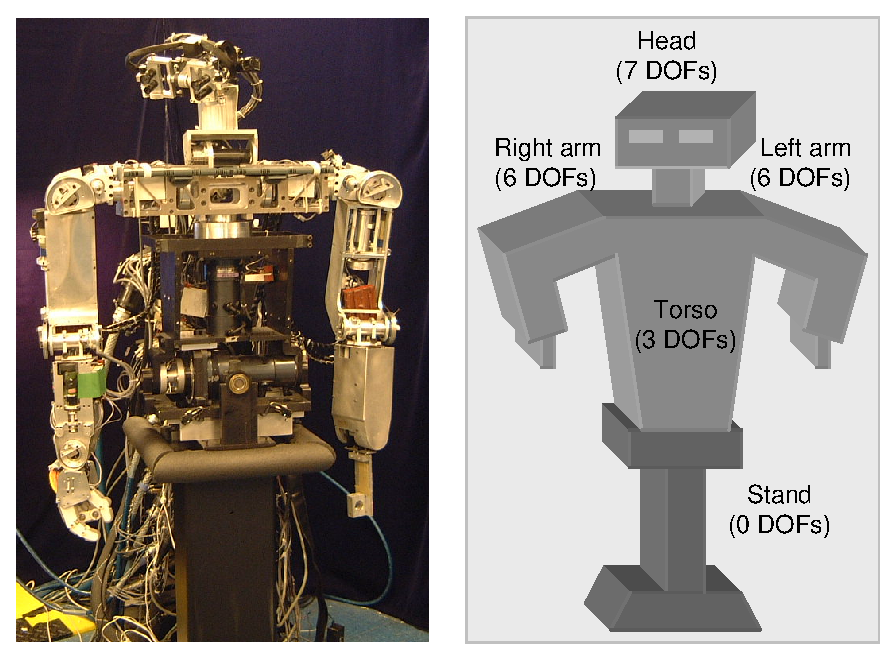
\psfig{file=cog-schematic.eps,height=2.5in,clip=,silent=}
}
\caption{ 
%
  Degrees of freedom (DOFs) of the robot Cog.  The arms terminate
  either in a primitive ``flipper'' or a four-fingered hand.  
\ifverbose
The hand
  is an independent research project by Matthew Marjanovi\'{c}, and
  will not be employed or described here.  
\fi
  The head, torso, and arms
  together contain 22 degrees of freedom.
%
}
\label{fig:cog-schematic}
\end{figure}


\ifverbose
\begin{figure}[tbh]
\begin{center}
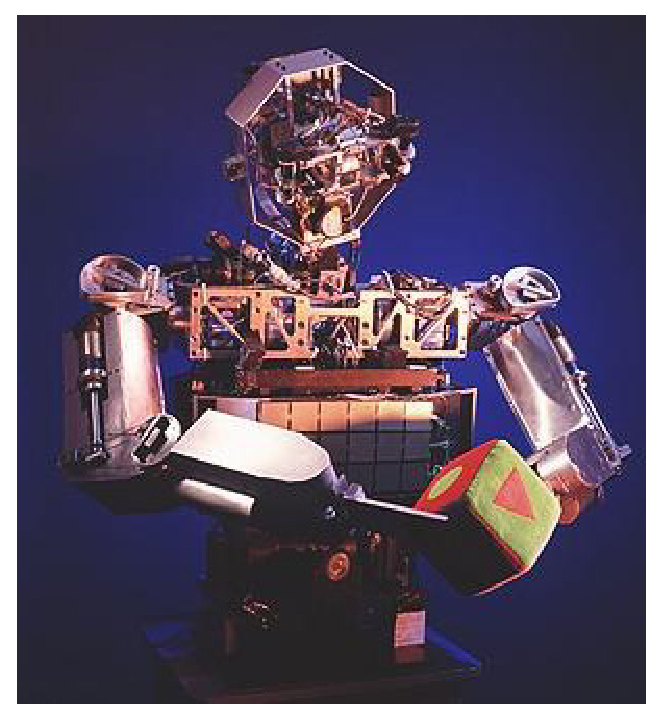
\includegraphics[height=3.5cm]{cog5-flip.eps}
\ \ \ \ 
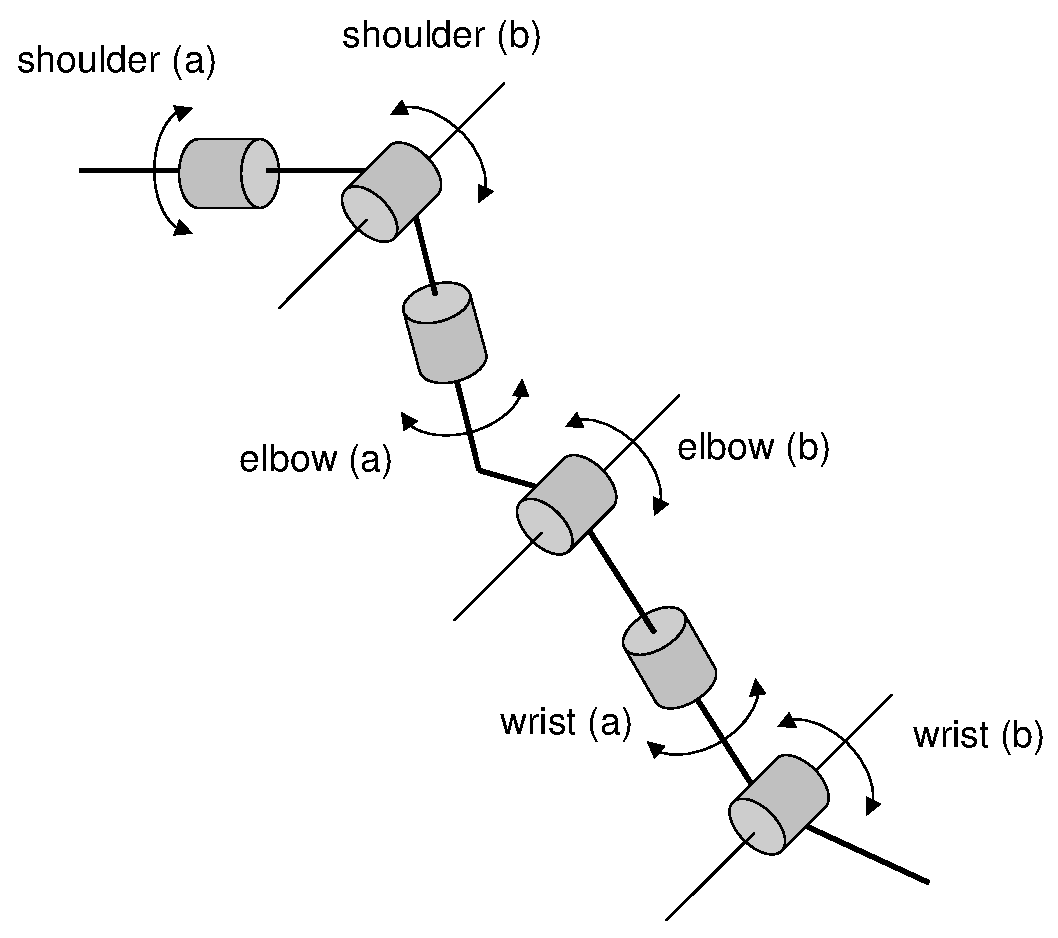
\includegraphics[height=3.5cm]{arm-motors.eps}
\caption{ 
\label{fig:arm-motors}
%
Kinematics of the arm, following \protect\cite{williamson99robot}.
There are a total of six joints, divided into a pair for each of
the shoulder, elbow, and wrist/flipper.
%
}
\end{center}
\end{figure}
\fi



\section{Perceiving direct effects of action}

Motion of the arm may generate optic flow directly through the
changing projection of the arm itself, or indirectly through an object
that the arm is in contact with.  While the relationship between the
optic flow and the physical motion is likely to be extremely complex,
the correlation in time of the two events will generally be
exceedingly precise.  This time-correlation can be used as a
``signature'' to identify parts of the scene that are being influenced
by the robot's motion, even in the presence of other distracting
motion sources.  In this section, we show how this tight correlation
can be used to localize the arm in the image without any prior
information about visual appearance.  In the next section we will show
that once the arm has been localized we can go further, and identify
the boundaries of objects with which the arm comes into contact.

\subsubsection*{Reaching out}

The first step towards manipulation is to reach objects within the
workspace.  If we assume targets are chosen visually, then ideally we
need to also locate the end-effector visually to generate an error
signal for closed-loop control.  Some element of open-loop control is
necessary since the end-point may not always be in the field of view
(for example, when it is in its the resting position), and the overall
reaching operation can be made faster with a feed-forward contribution
to the control.

\begin{figure}[tb]
\begin{center}
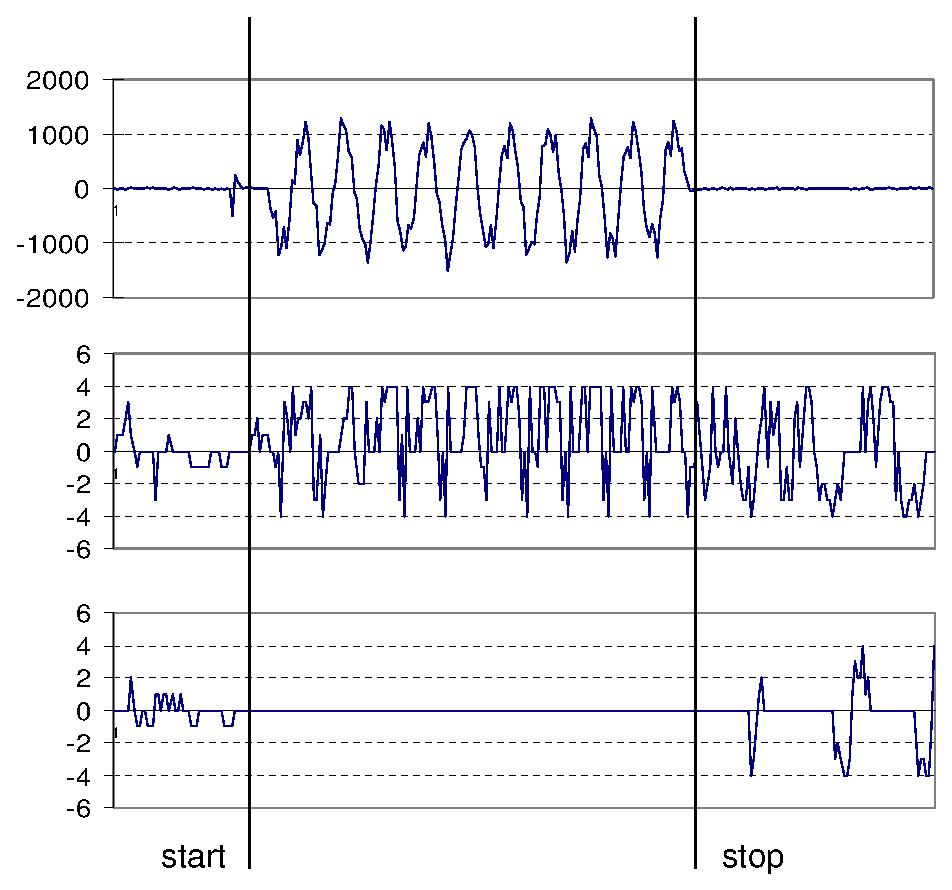
\includegraphics[width=\columnwidth]{joint-correlation2.eps}
\caption{ 
\label{fig:joint-correlation}
%
An example of the correlation between optic flow and arm movement.
The traces show the movement of the wrist joint (upper plot)
and optic flow sampled on the arm (middle plot) and away from it (lower
plot).  As the arm generates a repetitive movement, the oscillation
is clearly visible in the middle plot and absent in the lower.
Before and after the movement the head is free to saccade, generating the
other spikes seen in the optic flow.
%
}
\end{center}
\end{figure}


The simplest possible open loop control would map directly from a
fixation point to the arm motor commands needed to reach that point
\cite{metta99developmental} using a stereotyped trajectory, perhaps
using postural primitives \cite{mussa-ivaldi92vector}.  If we can
fixate the end-effector, then it is possible to to learn this map by
exploring different combinations of direction of gaze vs.  arm
position \cite{Marjanovic-96-SAB,metta99developmental}.  So locating
the end-effector visually is key both to closed-loop control, and to
training up a feed-forward path.  We shall demonstrate that this
localization can be performed without knowledge of the arm's appearance,
and without assuming that the arm is the only moving object in the
scene.

\ifverbose
NEW The closed loop control requires the identification of both the
end-effector and the target in the image plane. As in the visual
servoing literature \cite{espiau92new} it is certainly possible to
design a feedback controller based on the knowledge of the Jacobian
mapping between the image and the robot joint space -- globally
represented by both the position of the cameras in space and the arm.
The state space in our case is 13-dimensional. Constructing the
Jacobian requires the calibration of the robot and the estimation of
the kinematics.  On the other hand, for the configurations where the
object and the end-point are close one to the other, it is possible to
simplify the formulation by assuming the controller is locally
constant with respect to the arm position (this removes 6 dimensions).
Still the controller is a function of the configuration of the head.
This dependency must be roughly taken into account to move the arm
correctly. The requirements in terms of precision are in fact not that
stringent because what matters for the closed loop controller is that
the sign remains negative with respect to the visual error. For our
purpose this relationship can be learned by the same exploration
procedure mentioned above for the open loop controller.  For both
controllers the problem translates into localizing the arm's end-point
in the image plane. We shall demonstrate that visual localization can
be performed without relying on a particular color or pattern but
simply on movement and motor information.
\fi

\begin{figure}[tb]
\begin{center}
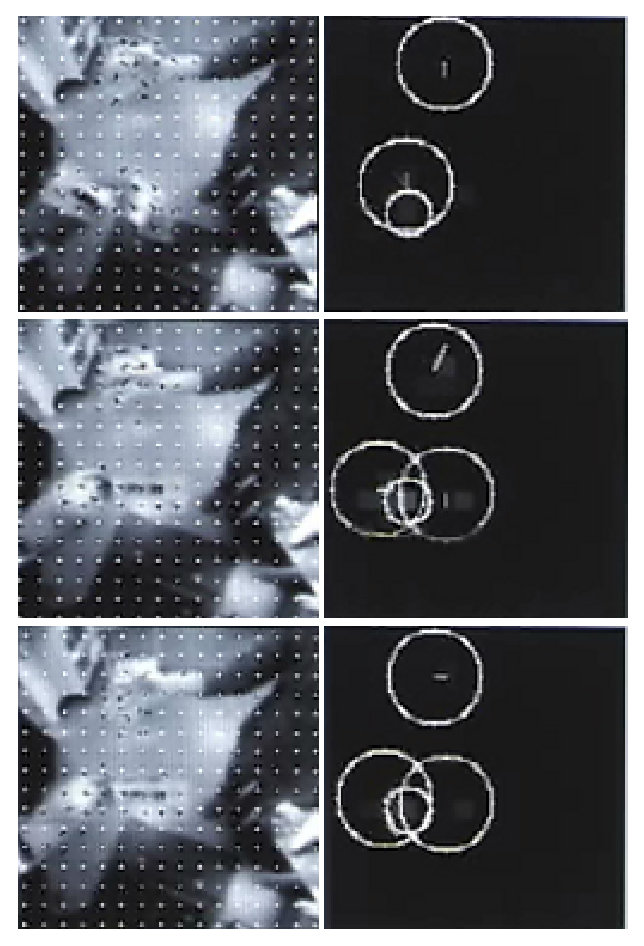
\includegraphics[width=6cm]{arm-detection2.eps}
\caption{ 
\label{fig:arm-detection}
%
Detecting the arm/gripper through motion correlation. The robot's
point of view and the optic flow generated are shown on the left. On
the right are the results of correlation.  Large circles represent the
results of applying a region growing procedure to the optic flow.
Here the flow corresponds to the robot's arm and the experimenter's
hand in the background. The small circle marks the point of maximum 
correlation, identifying the regions that correspond to the robot's own arm.
%
}
\end{center}
\end{figure}


\subsubsection*{Localizing the arm visually}

The robot is not a passive observer of its arm, but rather the
initiator of its movement.  This can be used to distinguish the arm
from parts of the environment that are more weakly affected by the
robot.  The arm of a robot was detected in \cite{Marjanovic-96-SAB} by
simply waving it and assuming it was the only moving object in the
scene.  We take a similar approach here, but use a more
stringent test of looking for optic flow that is correlated with
the motor commands to the arm.  This allows unrelated movement
to be ignored.  Even if a capricious engineer where to 
replace the robot's arm with one of a very different appearance,
and then stand around waving the old arm, this detection method
will not be fooled.  

The actual relationship between arm movements and the optic flow they
generate is complex.  Since the robot is in control of the arm, it can
choose to move it in a way that bypasses this complexity.  In
particular, if the arm rapidly reverses direction, the optic flow at
that instant will change in sign, giving a tight, clean temporal
correlation.  Since our optic flow processing is coarse (a $16\times
16$ grid over a $128\times 128$ image at 15 Hz), we simply repeat this
reversal a number of times to get a strong correlation signal during
training.  With each reversal the probability of correlating with
unrelated motion in the environment goes down.  This probability could
also be reduced by higher resolution (particularly in time) visual
processing.

\ifverbose
Localizing the robot arm is not the same as searching into the visual
space for a generic object we do not have any expectancy on its
whereabouts. The robot can exploit the fact it looks for its own body
part to self-generate useful cues to help the localization. The
fundamental idea is to cross-correlate the presence of motion in the
image with the actual arm motion as sensed through proprioception (or
efference copy). When the two quantities have a positive correlation
over a given time window, we can assert that that image location
belongs to the visual projection of the arm. From the visual point of
view, the optic flow can be used. We employed a block matching
technique over a 16x16 grid out of a 128x128 pixels image.
\fi


\begin{figure}[tb]
\begin{center}
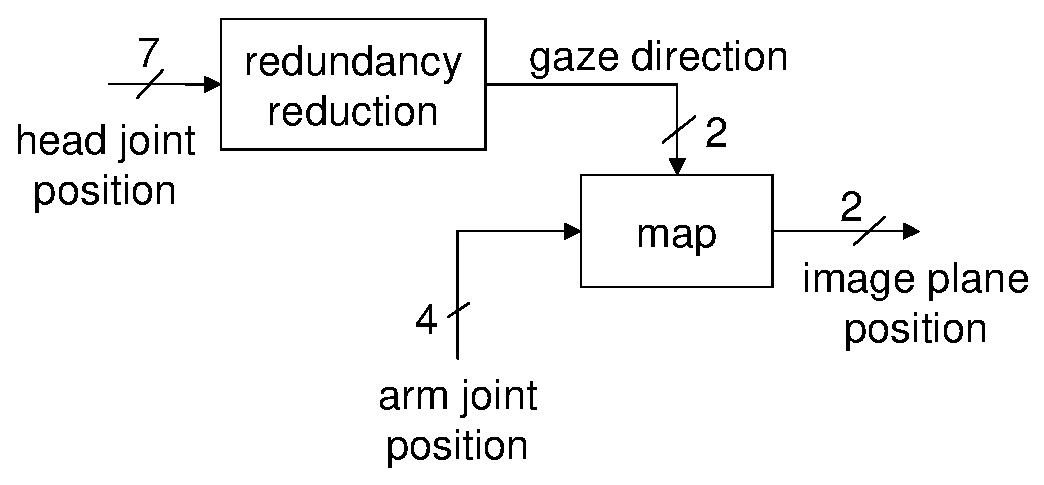
\includegraphics[width=\columnwidth]{mapping-reach.eps}
\caption{ 
\label{fig:mapping-reach}
%
Mapping from proprioceptive input to a visual prediction. Head and arm
joint positions are used to estimate the position of the projection of
the hand in the image plane.  Redundant configurations of the (7 DOF)
head are mapped to a simpler (2D) representation, and the wrist-related 
DOFs of the arm are ignored.
%
}
\end{center}
\end{figure}


\ifverbose
These two ideas were exploited contextually. The cross-correlation
runs on a 500ms time window while the robot generates a relatively
high-frequency movement. The resulting correlation array (each pixel
is correlated with all joints) is post-processed by a thresholding
procedure and subsequently by a region-growing algorithm. Regions are
identified and labeled. The arm position is identified as the center
of mass of the region containing the maximum of the correlation
function\iflong (see Figure~\ref{fig:arm-detection})\fi.
\fi

Figure~\ref{fig:joint-correlation} shows an example of this procedure
in operation, comparing the velocity of the arm's wrist with the optic
flow at two positions in the image plane.  A trace taken from a
position away from the arm shows no correlation, while conversely the
flow at a position on the wrist is strongly different from zero over
the same period of time.  Figure~\ref{fig:arm-detection} shows
examples of detection of the arm and rejection of a distractor.


\subsubsection*{Localizing the arm using proprioception}

The localization method for the arm described so far relies on a
relatively long ``signature'' movement that would slow down reaching.
This can be overcome by training up a function to estimate the
location of the arm in the image plane from proprioceptive information
(joint angles) during an exploratory phase, and using that to 
constrain arm localization during actual operation.
As a function approximator we simply fill a look-up table,
reducing the 11-dimensional input space of joint angles based on 
the much lower number of degrees of freedom used in controlling them
(see Figure~\ref{fig:mapping-reach}).
Figure~\ref{fig:predict-position} shows the resulting behavior
after about twenty minutes of real-time learning. 
%
\ifverbose
Note as both the
position of the arm and the direction of gaze change in these
examples: the position of objects such as the base of the robot at the
bottom of the image varies.
\fi
%
\ifverbose
We can imagine building a function from examples to predict the
position of the arm/end-point in the image plane. Examples are
collected when the arm is localized and have the form of joint
space-image coordinates [equation here?]. In principle a very big
lookup table can be used. The problem is that the input space is
13-dimensional (7 degrees of freedom describing the head configuration
and 6 describing the arm position), and nearest neighbor lookup tables
are known to work poorly in highly dimensional spaces. Beside,
collecting enough samples to span the space densely enough might
require a very long time. We can observe though that only the first
four arm joints determine the appearance of the end-point in the image
plane (the wrist is irrelevant), and the position in space of the
image plane although determined by the head configuration can be
described by only two numbers. These two parameters describe only the
orientation and not the position in space. In theory a distance factor
should be also considered, but it would only marginally influence the
map because the change in distance of the arm with respect to the
camera is small for the allowed movement of the head/arm [hope I
convinced the audience].
\fi


\ifverbose
Can we determine which is the set of redundant configuration of the
head for each given orientation of the camera? We can indeed spot when
two orientations of the camera are the same in spite of the head
configuration been different: this is true if the following statements
are true:
%
\begin{itemize}
%
\item Projection of the arm end-point in the image plane.
%
\item Arm joint position.
%
\item The head configurations are different.
%
\end{itemize}
%
Whenever a new data point (input/output) is used for training, it is
checked against all existing elements in the lookup table. If any of
them satisfy the above-mentioned conditions it is not inserted as a
new point but rather as belonging to the same camera direction.
Figure~\ref{fig:mapping-reach} depicts a schematic of the map as
implemented.

\fi

\ifverbose
\section{Putting things together}

Figure 6 shows how all components of the reaching subsystem are put
together. The lowest level controller is a double loop consisting of a
torque loop based on the reading of the joint strain gauges, and a
position/velocity feedback loop based on the potentiometer readings.
Depending on the tuning of the position/velocity gain it is possible
to obtain a low stiffness yet precise enough controller. Our tuning in
fact has a low positional gain and a relatively higher velocity gain.
The behavior is thus that of a low-stiffness controller with still a
good behavior when closing a velocity loop [unclear].

The successive level above is a simple linear combination of postural
primitives. There are four primitives in the present implementation,
which span a good portion of the arm workspace frontal to the robot
chest. Primitives are defined in joint space.

Oscillatory movements are generated by a specific subsystem in
parallel to the postural primitives block. Oscillations are created by
specifying directly the speed of the arm joints.

Further up in the control chain there is the open loop controller.
This is implemented as a nearest neighbor lookup table mapping the
gaze direction into a set of coefficient. The coefficients are the
weights of the linear combination of postural primitives.

The arm locator algorithms control in different ways both the
generation of appropriate movements for the self-localization and the
switching between different control regimes (not indicated in figure).

There are two caveats: first, an additional and more precise visual
bit of information is probably needed, and second, the closed loop
controller has not been implemented yet. The former issue can probably
be solved by looking for a gray blob close to the predicted arm
position. Once the position of the end-point is accurately estimated,
a reliable closed loop controller can be learned and employed after the
open loop to bring the flipper in contact with the target object.
\fi

\ifverbose
\begin{figure}[tbh]
\begin{center}
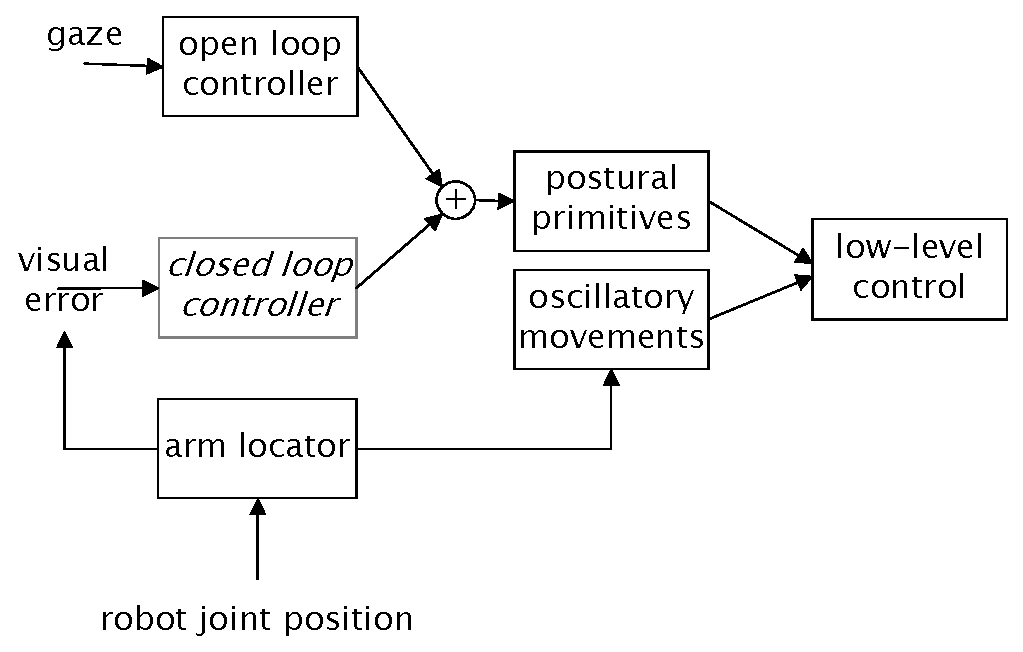
\includegraphics[width=\columnwidth]{control-flow.eps}
\caption{ 
\label{fig:control-flow}
%
  The controller.  Probably have to bring back text to describe this
  if we include this figure.
%
}
\end{center}
\end{figure}
\fi

\begin{figure}[tbh]
\begin{center}
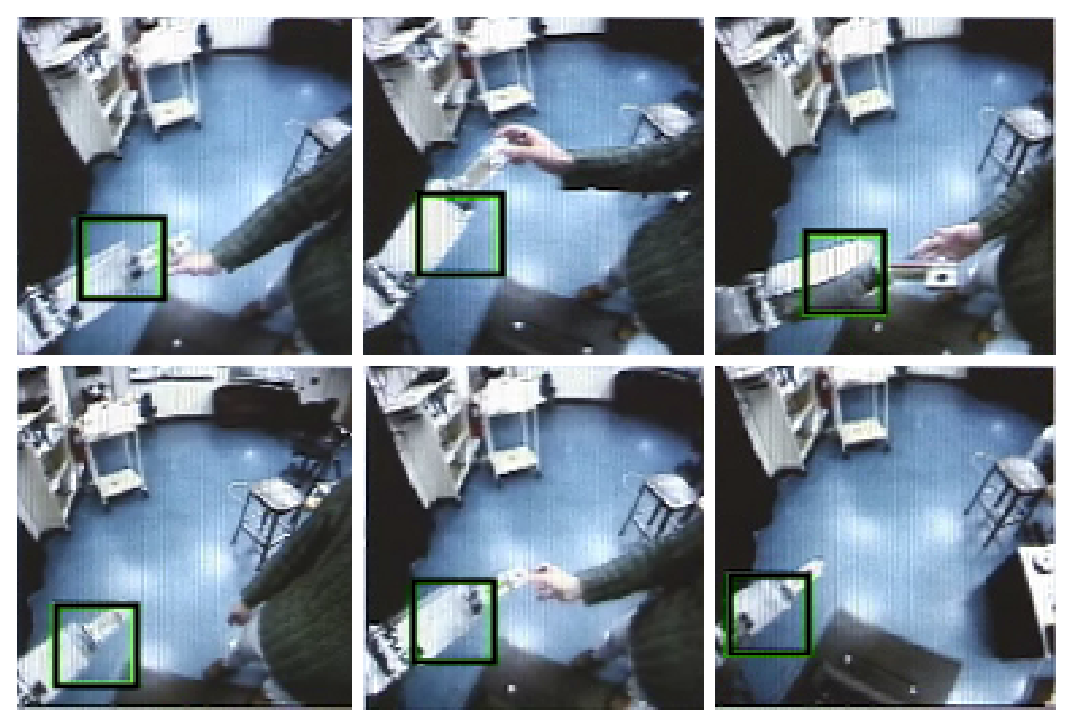
\includegraphics[width=\columnwidth]{predict-position.eps}
\caption{ 
\label{fig:predict-position}
%
Predicting the location of the arm in the image as the head and arm
change position. The rectangle represents the predicted position of
the arm using the map learned during a twenty-minute training run.
The predicted position just needs to be sufficiently accurate to
initialize a visual search for the exact position of the end-effector.
%
}
\end{center}
\end{figure}




\begin{figure*}[tbh]
\begin{center}
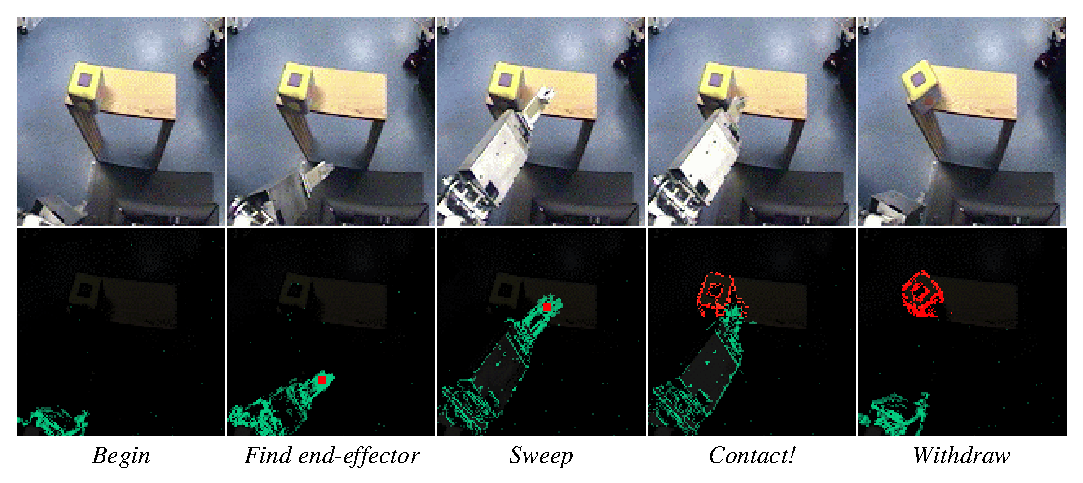
\includegraphics[width=\textwidth]{poking-sequence.eps}
%%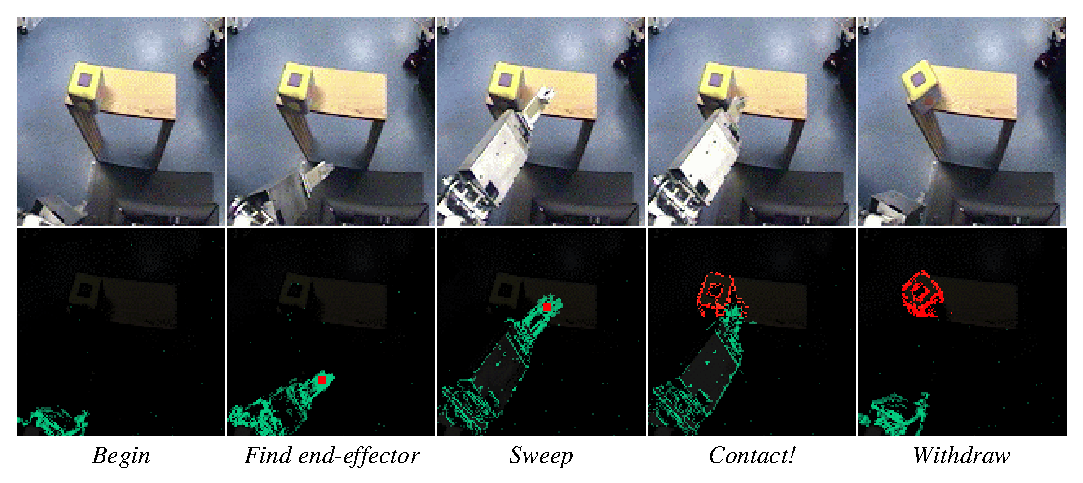
\includegraphics[width=14cm]{poking-sequence.eps}
\caption{ 
\label{fig:poking-sequence}
%
  The upper sequence shows an arm extending into a workspace, tapping
  an object, and retracting.  This is an exploratory mechanism for
  finding the boundaries of objects, and essentially requires the arm
  to collide with objects under normal operation, rather than as an
  occasional accident.  The lower sequence shows the shape
  identified from the tap using simple image differencing and flipper
  tracking.
%
}
\end{center}
\end{figure*}


\section{Perceiving indirect effects of action}

We have assumed that the target of a reaching operation is chosen
visually.  As discussed in the introduction, visual
segmentation is not easy, so we should not expect a target selected in
this way to be a correctly segmented.  For the example scene in
Figure~\ref{fig:setup-sequence} (a cube sitting on a table), the small
inner square on the cube's surface pattern might be selected as a
target.  The robot can certainly reach towards this target, but
grasping it would prove difficult without a correct estimate of the
object's physical extent.  In this section, we develop a procedure
for refining the segmentation using the same idea of correlated
motion used earlier to detect the arm.

When the arm enters into contact with an object, one of several
outcomes are possible.  If the object is large, heavy, or otherwise
unyielding, motion of the arm may simply be resisted without any
visible effect.  Such objects can simply be ignored, since the robot
will not be able to manipulate them.  But if the object is smaller, it
is likely to move a little in response to the nudge of the arm.  This
movement will be temporally correlated with the time of impact, and
will be connected spatially to the end-effector -- constraints that
are not available in passive scenarios~\cite{birchfield99depth}.  If
the object is reasonably rigid, and the movement has some component in
parallel to the image plane, the result is likely to be a flow field
whose extent coincides with the physical boundaries of the object.

Figure~\ref{fig:poking-sequence} shows how a ``poking'' movement can
be used to refine a target.  During a poke operation, the arm begins
by extending outwards from the resting position.  The end-effector (or
``flipper'') is localized as the arm sweeps rapidly outwards, using
the heuristic that it lies at the highest point of the region of optic
flow swept out by the arm in the image (the head orientation and
reaching trajectory are controlled so that this is true).  The arm is
driven outward into the neighborhood of the target which we wish to
define, stopping if an unexpected obstruction is reached.  If no
obstruction is met, the flipper makes a gentle sweep of the area
around the target.  This minimizes the opportunity for the motion of
the arm itself to cause confusion; the motion of the flipper is
bounded around the endpoint whose location we know from tracking
during the extension phase, and can be subtracted easily.  Flow not
connected to the end-effector can be ignored as a distractor.  

For simplicity, the head is kept steady throughout the poking
operation, so that simple image differencing can be used to detect
motion at a higher resolution than optic flow.  Because a poking
operation currently always starts from the same location, the arm
is localized using a simple heuristic rather than the procedure described
in the previous section -- the first region of optic flow appearing
in the lower part of the robot's view when the reach begins
is assumed to be the arm.

\begin{figure}[tbh]
\begin{center}
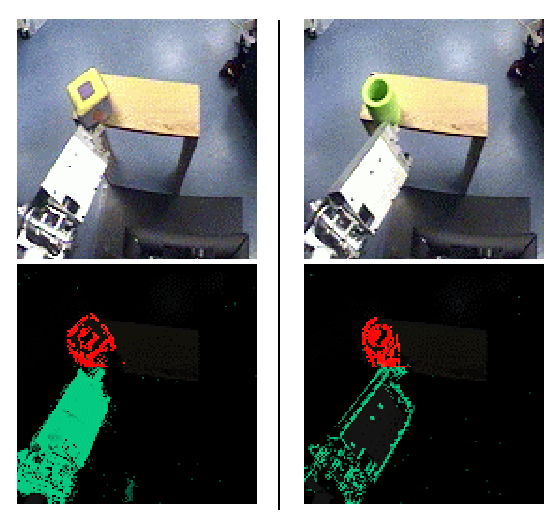
\includegraphics[width=\columnwidth]{cube-and-cylinder.eps}
\caption{ 
\label{fig:cube-and-cylinder}
%
  Poking can reveal a diffence in the shape of two objects without
  any prior knowledge of their appearance.
%
}
\end{center}
\end{figure}

The poking operation gives clear results for a rigid object that is
free to move.  What happens for non-rigid objects and objects that are
attached to other objects?  Here the results of poking are likely to
be more complicated to interpret -- but in a sense this is a good
sign, since it is in just such cases that the idea of an object
becomes less well-defined.  Poking has the potential to offer an
operational theory of ``objecthood'' that is more tractable than a
vision-only approach might give, and which cleaves better to the true
nature of physical assemblages.  The idea of a physical object is
rarely completely coherent, since it depends on where you draw its
boundary and that may well be task-dependent.  Poking allows us to
determine the boundary around a mass that moves together when
disturbed, which is exactly what we need to know for manipulation.  As
an operational definition of object, this has the attractive property
of breaking down into ambiguity in the right circumstances -- such
as for large interconnected messes, floppy formless ones, liquids,
and so on.



\section{Developing mirror neurons?}

\begin{figure}[tb]
\begin{center}
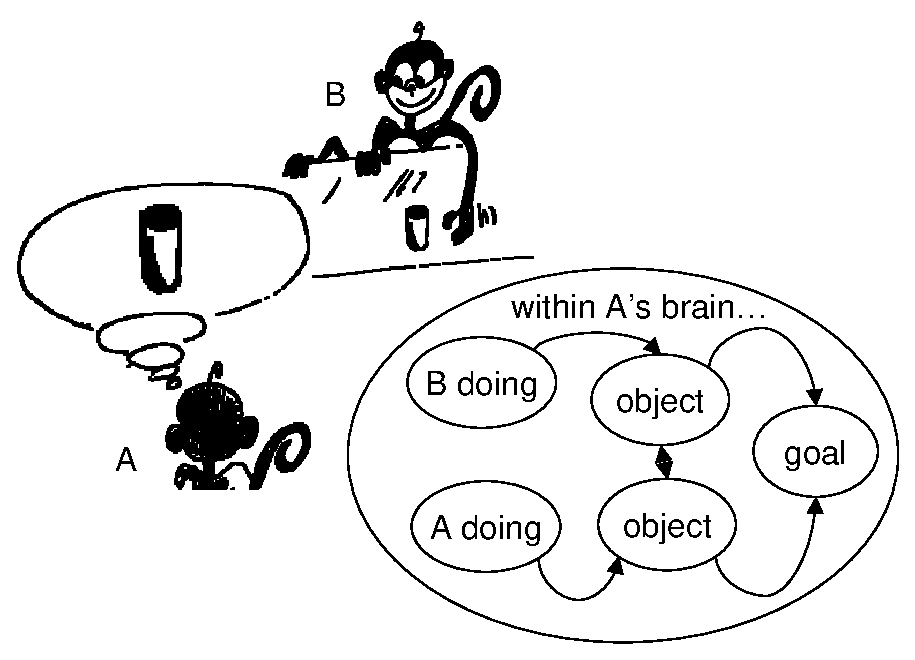
\includegraphics[width=\columnwidth]{mirror-monkey.eps}
\caption{ 
\label{fig:mirror-monkey}
%
Mirror neurons and causality: from the observer's point
of view (A), understanding B's action means mapping it onto the
observer's own
motor repertoire. If the causal chain leading to the goal is already
in place (lower branch of the graph) then the acquisition of a
mirror neuron for this particular action/object is a matter of
building and linking the upper part of the chain to the lower one.
There are various opportunities to reinforce this link either at the object
level, at the goal level or both. 
%%Developmentally we can explain
%%mirror neurons only if we take into account another class of neurons
%%(called canonical) which in practice describes the lower branch of the
%%graph.
%
}
\end{center}
\end{figure}

\ifverbose
The latest instantiation of the ``general principle'' we would like to
dwell upon is related to mirror neurons. It turns out that the causal
chain here is more compliceted. This requires a more complicated
structure to support it.
\fi

Poking moves us one step outwards on a causal chain away from the
robot and into the world, and gives a simple experimental procedure
for segmenting objects.  There are many possible elaborations of this
method (some are mentioned in the conclusions), all of which lead to a
vision system that is tuned to acquiring data about an object by
seeing it manipulated by the robot.  An interesting question then is
whether the system could extract useful information from seeing an
object manipulated by someone else.  In the case of poking, the robot
needs to be able to estimate the moment of contact and to track the arm
sufficiently well to distinguish it from the object being poked.  We
are interested in how the robot might learn to do this.  One approach
is to chain outwards from an object the robot has poked.  If someone
else moves the object, we can reverse the logic used in poking --
where the motion of the manipulator identified the object -- and
identify a foreign manipulator through its effect on the object.
Poking is an ideal testbed for future work on this, since it is much
simpler than full-blown object manipulation and would only require a
very simple model of the foreign manipulator to work.

There is considerable precedent in the literature for a strong
connection between viewing object manipulation performed by either
oneself or another \cite{wohlsclager02human}.  As we already mentioned
F5 contains a class of neurons called canonical neurons that have a
very specific response when an object is being either manipulated or
fixated.  Grossly simplifying, we might think of canonical neurons as
an association table of grasp/manipulation (action) types with object
(vision) types.  Another class of neurons called ``mirror neurons''
can then be thought of as a second-level association map which links
together the observation of a manipulative action performed by
somebody else with the neural representation of one's own action.

Figure~\ref{fig:mirror-monkey} shows this causal chain in action.
There are a series of interesting behaviors that can be realized based
on mirror neurons. Mimicry is an obvious application, since it
requires just this type of mapping between other and self in terms of
motor actions.  Another important application is the prediction of
future behavior from current actions, or even inverting the causal
relation to find the action that most likely will get to the desired
consequence.

\ifverbose

for example, by observing the part of an action the robot or the
bioagent can come out with suitable expectations of the consequences
of that action. On the other hand, the inverse behavior can also be
foreseen. The latter account to inverting the causal relation and
getting the action that most likely will get to the desired
consequence.

It might be argued that we need a two stages procedure to learn a
mirror representation, where we first learn ``something'' and only
subsequently we ``understand'' other people's behavior. The actual
developmental course might not be such artificially staged. A slight
advantage must be given though to the initial step of self-learning,
the undestanding comes later.


This set of associations can be learnt autonomously (by a robot for
example) simply by a trial and error procedure and possibly with a
reinforcing signal to tell when a given grasp/manipulatory gesture was
successful if applied to a particular object.

We should not probably think of this association as describing in
detail the object being manipulated visually. Perhaps only features
relevant to manipulation are stored (e.g. size, orientation in space).
This representation is a ``pragmatic'' one describing only those
properties of objects are needed to apply a particular set of actions
to them. Affordances are a good psychological analogue of F5
canonical neurons.
\fi


\ifverbose
How does this relate to causation?  The two situations in some sense
share the same goal, and more practically share the same object.  The
whole procedure assumes a basic discrimination of size and shape of
objects (not necessarily categorization in traditional sense), and the
exploitation of the visual information to the understanding of the
grasp type. In some cases though the goal might be unambiguous, e.g. a
needle is very unlikely grasped with a full palm grasp, as well as a
box is not grasped with a pinch grip. These are the most informative
allowing for the best discrimination of action type from the visual
perspective.
\fi

\ifverbose
The definition of imitation we gave here implicitly focus on imitating
the goal rather than the precise trajectory. This automatically takes
into account any difference in body structure between the actor and
the observer.

Of course, manipulation as in poking can lead to a better
understanding of the physical properties of objects not directly
amenable to visual exploration such as mass, roughness, softness, etc.
\fi

\begin{figure}[tbh]
\begin{center}
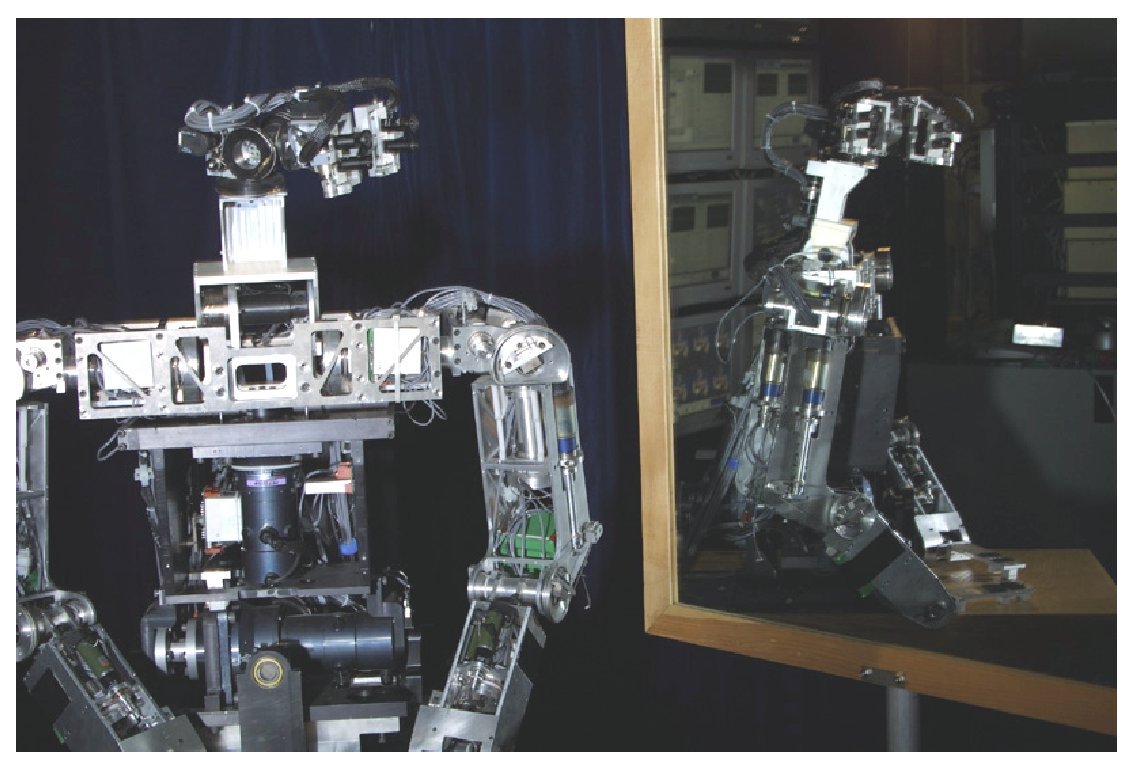
\includegraphics[width=\columnwidth]{mirror-cog.eps}
\caption{ 
\label{fig:mirror-cog}
%
The ultimate goal of this work is for our robot to follow chains of
causation outwards from its own simple body into the complex world.
%
}
\end{center}
\end{figure}




%%
\newcommand{\dgrs}{$^{\circ}$}

\section{Relative pose tracking}

We have seen that a gentle tap can be enough to reveal the outline of
an object in the image plane.  For very asymmetric objects, the
outline can be enough to greatly constrain their 3D pose.  For more
symmetric objects, the outline is not enough, and appearance or
tactile information needs to be considered.  Such information is
likely to be available only sporadically, depending on whether particular
surface features or in view or whether the robot arm is in contact
with the object.  This section describes a pose representation
that is well suited to ``piece-meal'' approaches.

We can decompose the three-dimensional processes involved in
determining the appearance of an object into an interaction between
two 2D objects: the image plane, and the surface of the object.  At
any moment, some set of surface patches on the object will be parallel
to the image plane.  As the object rotates in depth, different patches
become parallel.  When the object translates, or rotates in plane, the
parallel patches remain constant.  Figure~\ref{fig:tracking-dofs}
shows this decomposition.

\begin{figure}[tbp]
\centerline{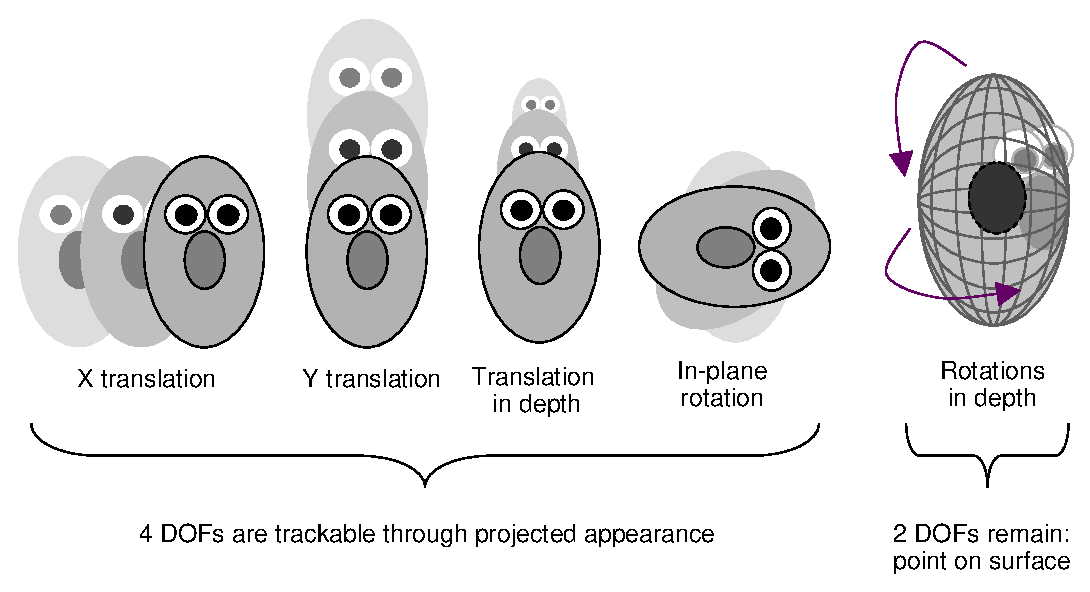
\includegraphics[width=\columnwidth]{tracking-dofs.eps}}
\caption{ 
%
  Two-dimensional tracking; four degrees of freedom are straightforward,
  but the last two are a little trickier.
%
}
\label{fig:tracking-dofs}
\end{figure}


\subsection{Current results}

The system has so far been tested on a data-set made available by
Sclaroff et al~\cite{lacascia00fast}, consisting of video of head
movements with ground truth measured by a Flock of Birds sensor on the
subjects' heads.  These sequences are 200 frames in duration.  To test
the stability of the tracker over long intervals, the Sclaroff
sequences are here artificially extending by looped them forward and
back for twenty iterations.  Angular measurements are limited by the
accuracy with which they can be initialized, which turns out to be to
within about 5\dgrs\ for roll and yaw, and about 10\dgrs\ for pitch.

\begin{figure}[tbp]
\centerline{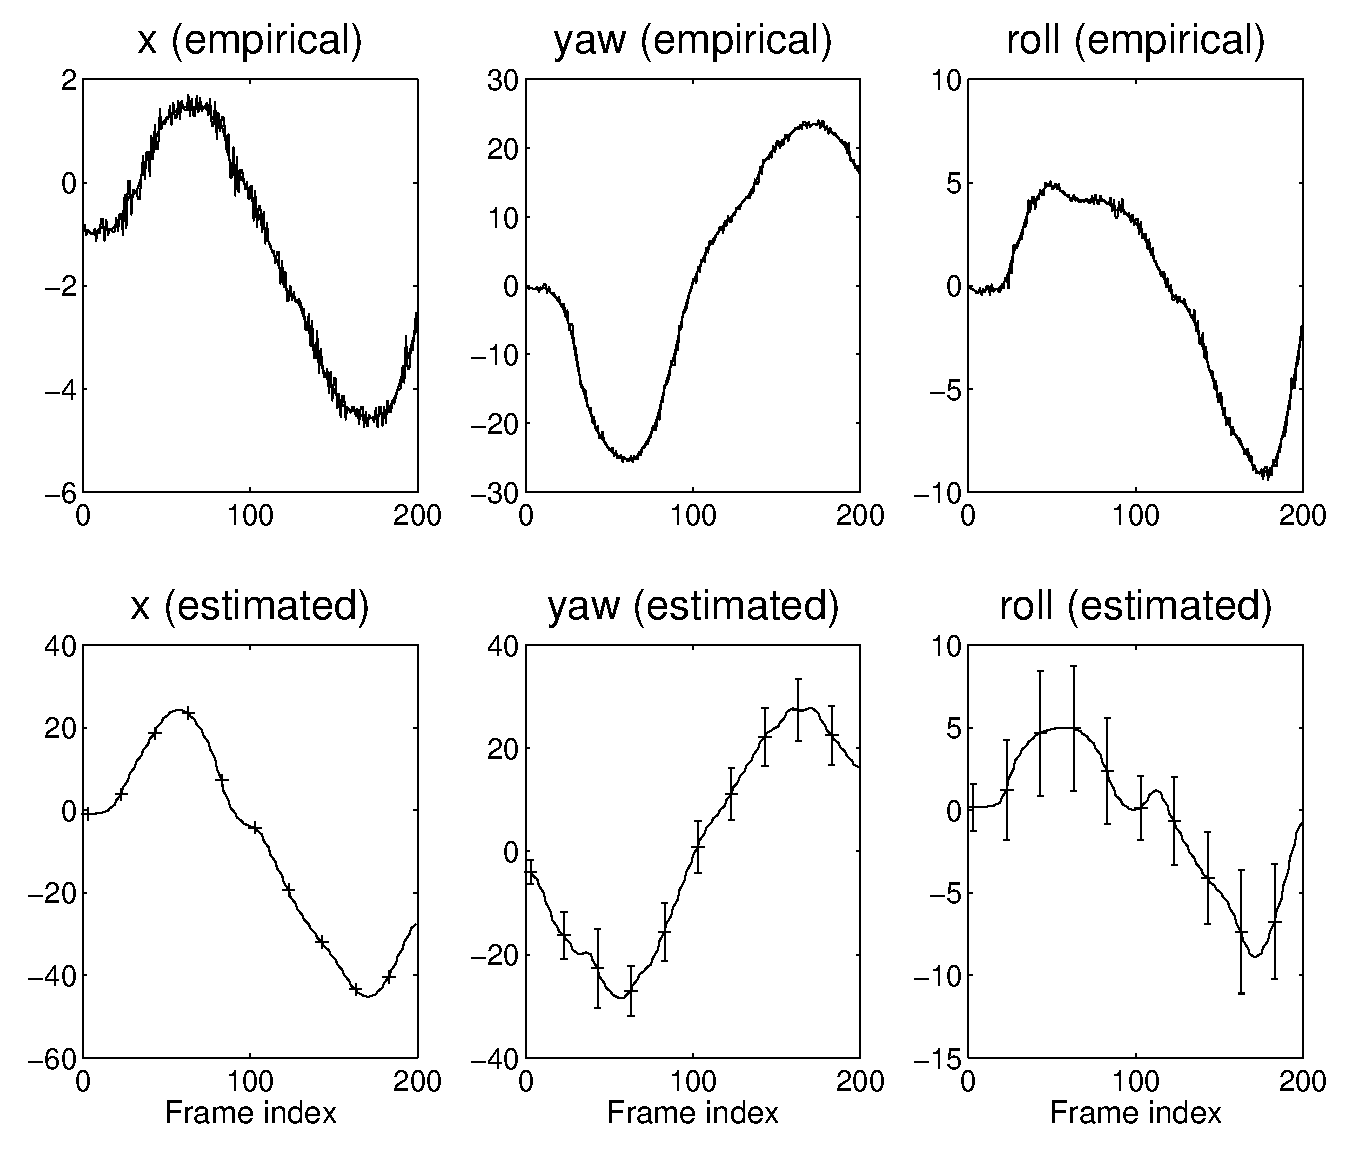
\includegraphics[width=\columnwidth]{yaw-roll-result.eps}}
\centerline{
\includegraphics[width=\columnwidth]{yaw-extremes.eps}}
\caption{ 
%
  Results for a sequence containing a yaw movement and horizontal
  translation, with all other parameters remaining basically unchanged
  except for a slight roll.  The top row shows ground truth.  The
  second row shows the estimated pose parameters that change
  significantly during the sequence.  The estimated $x$ coordinate is
  left in terms of the image plane.  Values plotted are averaged for
  each occurrence of a particular frame over a {\em single tracking
    run} constructed from a 200-frame sequence being played, then
  played in reverse, then repeated again for twenty iterations.  Error
  bars show the standard deviation of estimates for each frame.
%
}
\label{fig:yaw-roll-result}
\end{figure}



\section{Discussion and Conclusions}

In this paper, we showed how causality can be probed at different
levels by the robot.  Initially the environment was the body of the
robot itself, then later a carefully circumscribed interaction with
the outside world.  This is reminiscent of Piaget's distinction
between primary and secondary circular
reactions~\cite{ginsburg78piaget}.  Objects are central to interacting
with the ouside world.  We raised the issue of how an agent can
autonomously acquire a working definition of objects. 

\ifverbose
According to
recent neuroscience results the problem is ``well posed'' only if the
agent is embodied.
\fi

\ifverbose
We also 
the concept of causality and to a certain extent
our particular implementation fit well with a bulk of neural science
results. Implementing a model of development might help to 
understand ``how the brain does it''.
\fi


In computer vision there is much to be gained by bringing a
manipulator into the equation.  Many variants and extensions to the
experimental ``poking'' strategy explored here are possible.  For
example, a robot might try to move an arm around {\em behind} the
object.  As the arm moves behind the object, it reveals its occluding
boundary.  This is a precursor to visually extracting shape
information while actually manipulating an object, which is more
complex since the object is also being moved and partially occluded by
the manipulator.  Another possible strategy that could be adopted as a
last resort for a confusing object might be to simply hit it firmly,
in the hopes of moving it some distance and potentially overcoming
local, accidental visual ambiguity.  Obviously this strategy cannot
always be used!  But there is plenty of room to be creative here.



%The number of papers written on techniques for visual segmentation is
%vast.  Methods for characterizing the shape of an object through
%tactile information are also being developed, such as shape from
%probing \cite{cole87shape,paulos99fast} or pushing
%\cite{moll01reconstructing,jia98observing}.  But while it has long
%been known that motor strategies can aid
%vision~\cite{ballard91animate}, work on active vision has focused
%almost exclusively on moving cameras.  There is much to be gained by
%bringing a manipulator into the equation, as we have shown in this
%paper.  Many variants and extensions to the experimental ``poking''
%strategy explored here are possible.  For example, a robot might try
%to move an arm around {\em behind} the object.  As the arm moves
%behind the object, it reveals its occluding boundary.  This is a
%precursor to visually extracting shape information while actually
%manipulating an object, which is more complex since the object is also
%being moved and partially occluded by the manipulator.  Another
%possible strategy that could be adopted as a last resort for a
%confusing object might be to simply hit it firmly, in the hopes of
%moving it some distance and potentially overcoming local, accidental
%visual ambiguity.  Obviously this strategy cannot always be used!  But
%there is plenty of room to be creative here.





% thanks to many people...


\iflong
\section*{Acknowledgements}
\else
\begin{Acknowledgment}
\fi

This work benefited from discussions with Charles Kemp and Giulio
Sandini.  Many people have contributed to developing the Cog platform
\cite{brooks99cog}.  Funds for this project were provided by DARPA as
part of the ``Natural Tasking of Robots Based on Human Interaction
Cues'' project under contract number DABT 63-00-C-10102, and by the
Nippon Telegraph and Telephone Corporation as part of the NTT/MIT
Collaboration Agreement.

\iflong
\else
\end{Acknowledgment}
\fi


% and the bibliography:

\ifverbose

\nocite{ballard91animate}
\nocite{moll01reconstructing}
\nocite{paulos99fast}
\nocite{cole87shape}
\nocite{williamson99robot}
\nocite{brooks99cog}
\nocite{jia98observing}
\nocite{birchfield99depth}


\nocite{berkeley72new}
\nocite{kovacs00human}
\nocite{ungerleider82two}
\nocite{milner95visual}
\nocite{jeannerod97cognitive}
\nocite{rizzolatti88functional}
\nocite{gibson77theory}
\nocite{fadiga00visuomotor}
\nocite{rizzolatti98language}
\nocite{fogassi96coding}
\nocite{metta99developmental}
\nocite{espiau92new}
\nocite{mussa-ivaldi92vector}

\fi

{
\iflong
%%\footnotesize
\bibliographystyle{sab}
\else
\bibliographystyle{plain}
\fi
\bibliography{vision}
}

%\begin{thebibliography}{99}
%\bibitem{Einstein}A.\ Einstein: ``A theory of relativity''
% more articles
%\end{thebibliography}




\section{Extras}


\begin{figure}[tbh]
  \begin{center}
    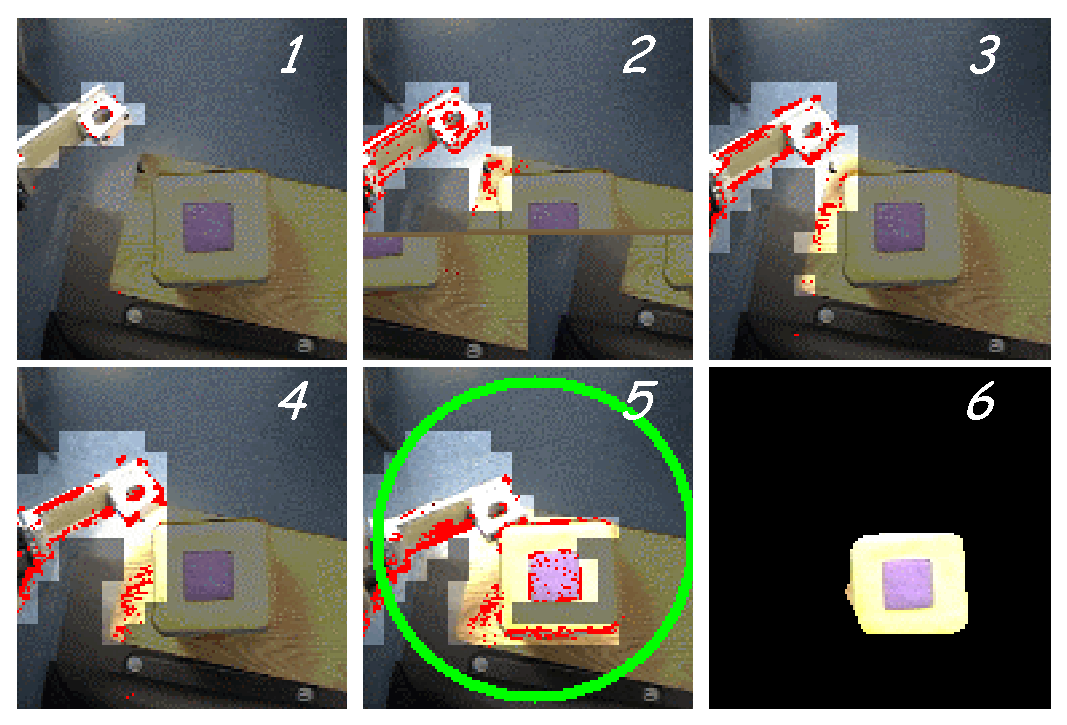
\includegraphics[width=2in]{collision-detail}
    \hspace{1in}
    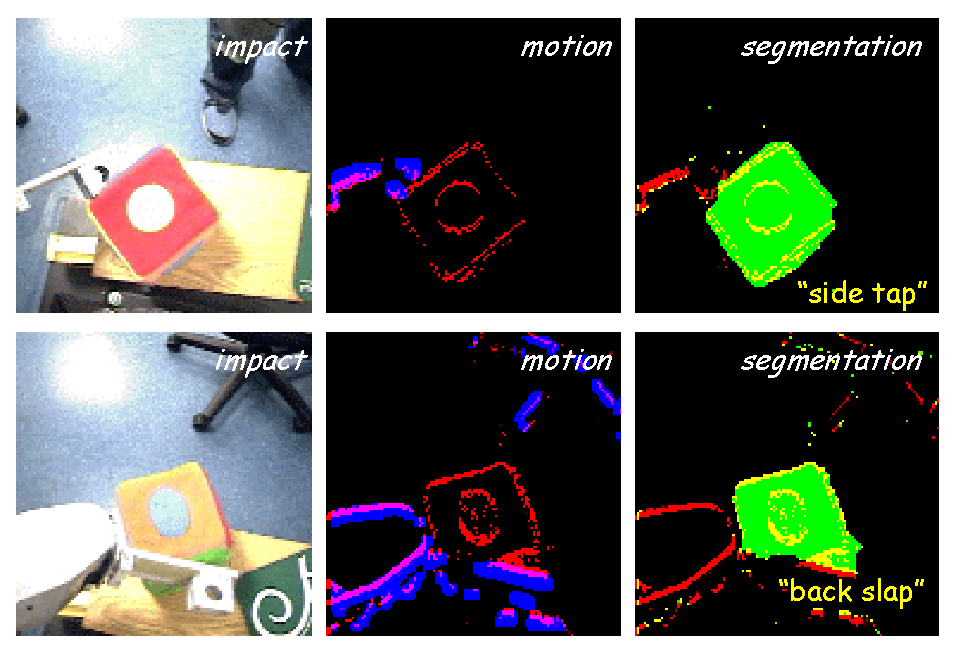
\includegraphics[width=2in]{segmentation-detail}
  \end{center}
  \caption{Part of the process}
\end{figure}

\begin{figure}[tbh]
  \centerline{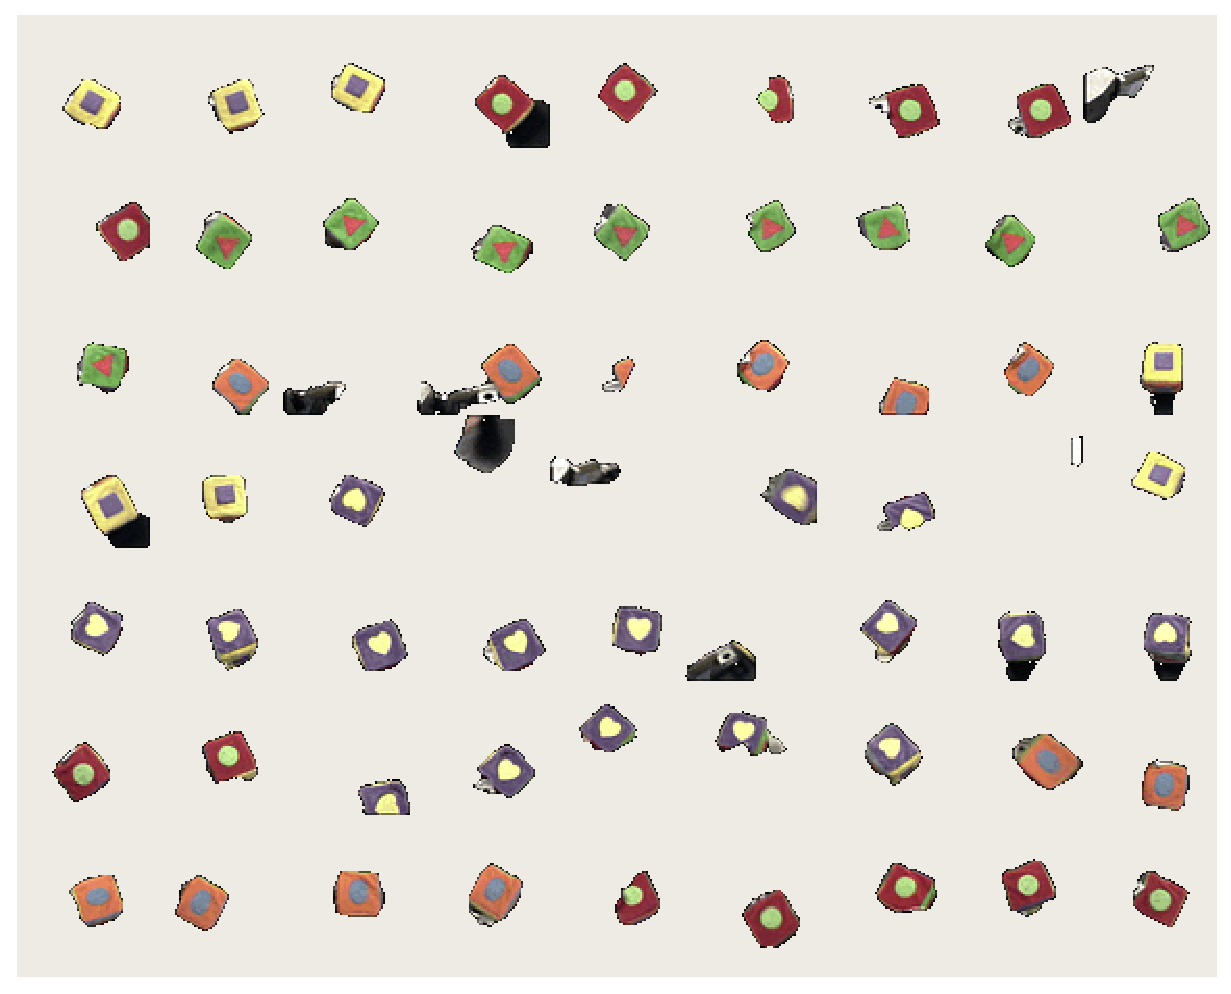
\includegraphics[width=2.5in]{experiment-montage}}
  \caption{Sample results}
  \label{fig:sample-results}
\end{figure}

\begin{figure}[tbh]
  \centerline{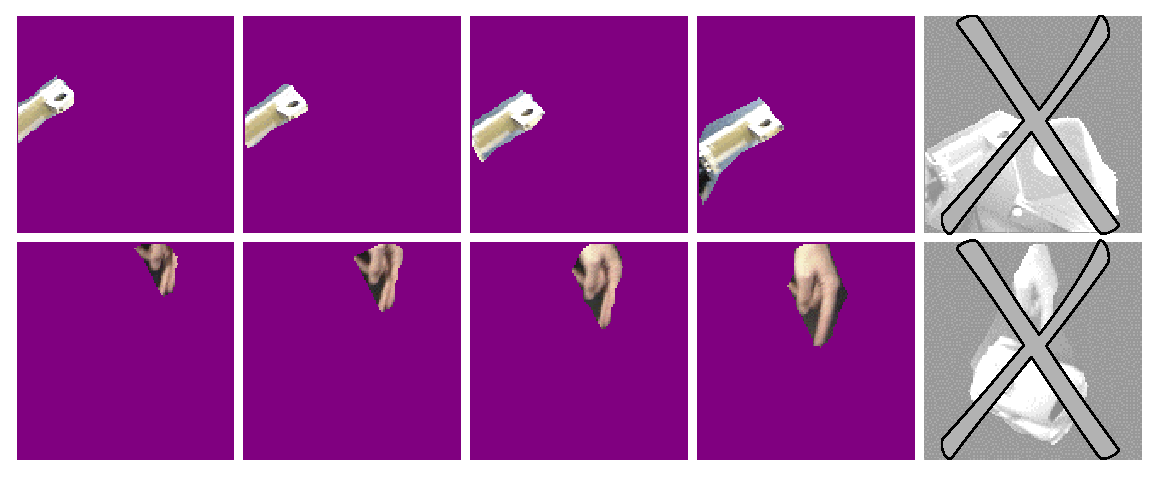
\includegraphics[width=2.5in]{manipulator-segment}}
  \caption{Segmenting the manipulator} 
  \label{fig:manipulator}
\end{figure}

\begin{figure}[tbh]
  \centerline{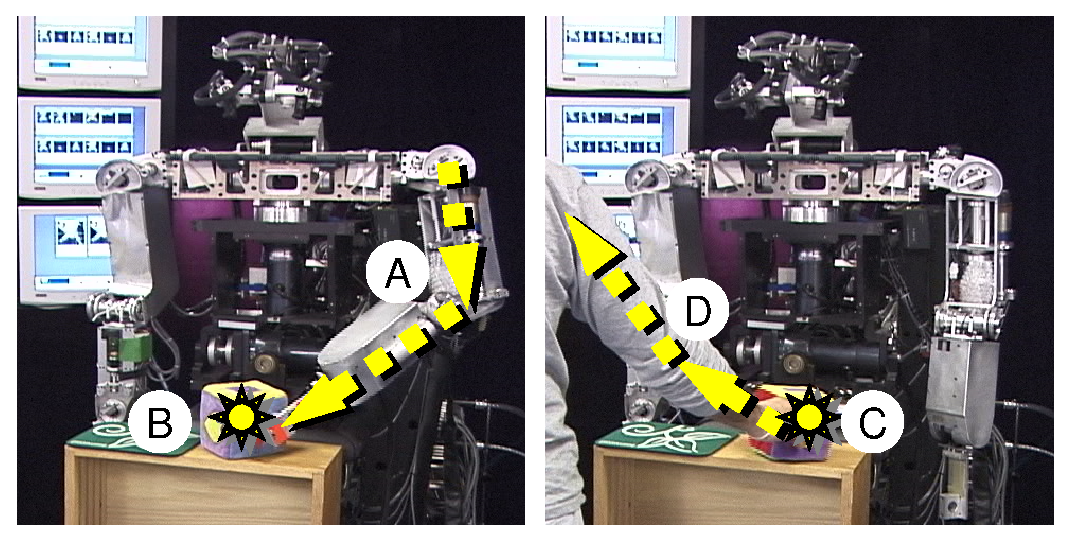
\includegraphics[width=2.5in]{tracing_causes}}
  \caption{foo} 
  %%\label{fig:foo}
\end{figure}


\begin{figure}[tbh]
  \centerline{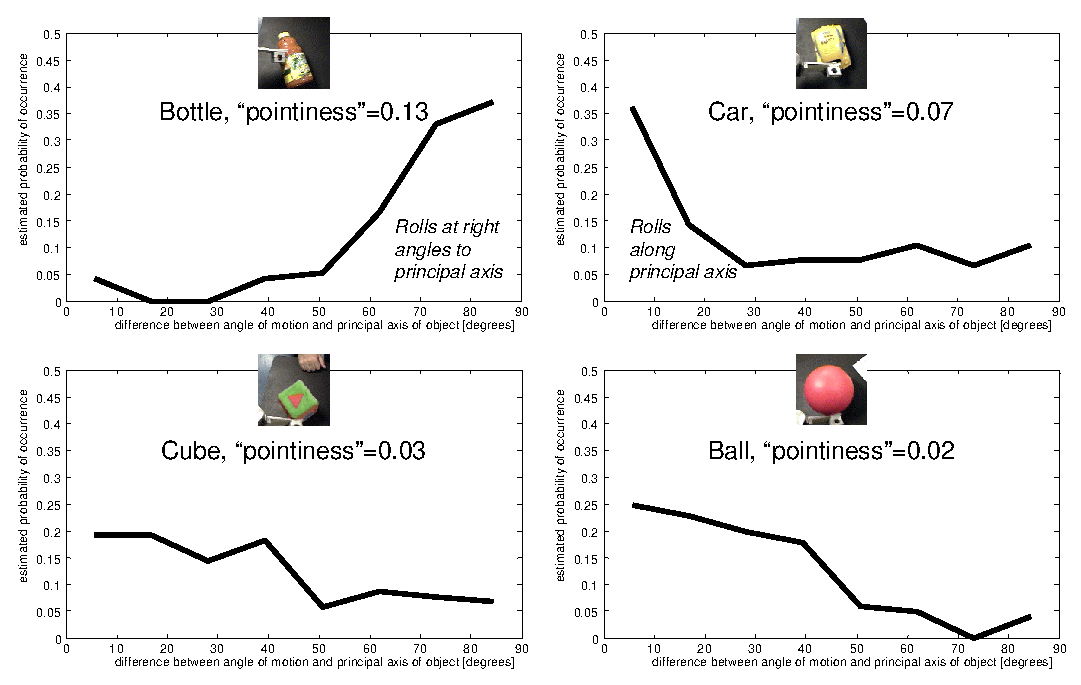
\includegraphics[width=2.5in]{rolling-graphs}}
  \caption{foo} 
  %%\label{fig:foo}
\end{figure}




\end{document}

% and never mind LaTeX's hysterical warnings about missing fonts... everything's fine!
